\documentclass[a4paper, 11pt]{article}	%Tipo de documento y opciones.

\usepackage[spanish]{babel}				%Idioma en el que se va a escibir.
\usepackage[utf8]{inputenc}				%Reconocimiento de caracteres como tildes.
\usepackage{fancyhdr}					%Paquete usado para la cabecera y el pie de página.
\usepackage{graphicx}					%Importar imágenes.
\usepackage{float}						%Posicionamiento de imágenes.

%Creamos comandos para los autores.
\newcommand{\enriquename}{Enrique Cabrerizo Fernández}
\newcommand{\guillermoname}{Guillermo Ruiz Álvarez}

\title{Práctica 3\\Redes de computadores}						%Título.
\author{\enriquename \and \guillermoname}						%Autores.
\date{14/11/2013}												%Fecha.

\pagestyle{fancyplain}					%Estilo: Usar cabeceras.
\fancyhf{}								%Borrar formato estándar.
\lhead{ \fancyplain{}{\enriquename} }	%Nombre de Enrique a la izquierda de la cabecera.
\rhead{ \fancyplain{}{\guillermoname} }	%Nombre de Guillermo a la derecha de la cabecera.
\cfoot{ \fancyplain{}{\thepage} }		%Número de la página centrada en el pie.

\begin{document}		%Comienza documento.
\maketitle			%Página de título.
\newpage				%Salto de página.
\tableofcontents		%Página de índice.
\newpage				%Salto de página.

\section{Introducción}	%Sección de introducción
En esta prática se va a implementar un programa que analizará y caracterizará una captura de paquetes de red. Para ello, utilizará un fichero \textit{*.pcap} que contenga una traza o directamente una interfaz especificada, dependiendo del argumento utilizado (véase sección \ref{sec:manual}, página \pageref{sec:manual}).
\\\\
Las funciones que realizará el programa son las siguientes:
\begin{itemize}
\item Mostrar por pantalla los porcentajes de paquetes IP, no ETH-IP, TCP, UDP y no TCP-UDP.
\item Mostrar por pantalla el top de 5 direcciones IP activas y el top de 5 puertos activos  (ambos por paquetes y tamaño en bytes).
\item Almacene en fichero y calcule el ECDF de la variable \textit{tamaño de paquete capturado}.
\item Almacene en fichero el ancho de banda a nivel 2 cada segundo por sentido.
\item Almacene en fichero y calcule el ECDF de la variable \textit{tiempo entre llegadas de los paquetes de un flujo entre un par de puertos}.
\end{itemize}

Adicionalmente se calcularán histogramas de las variables en las que se pide calcular un ECDF para así disponer de más información para analizar los datos.

De forma particular, el análisis que se va a llevar a cabo consistirá en mostrar la funcionalidad de la herramienta sobre el fichero proporcionado con el enunciado de la práctica: \textit{$practica3\_ rc1lab.pcap$}

\section{Análisis de la traza}
\subsection{Porcentajes de protocolos}
En la \textbf{Figura \ref{fig:recuento}} se muestran los porcentajes de los paquetes IP, no Eth-IP, UDP, TCP y no UDP-TCP.

%Inclusion de imagen.
\begin{figure}[H]
\centering
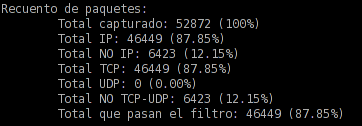
\includegraphics[width=0.8\textwidth]{recuento.png}
\caption{Recuento y porcentajes de protocolos de paquetes.}
\label{fig:recuento}
\end{figure}

Se puede observar que el $12,15\%$ de los paquetes (6423 paquetes) no son Eth-IP. Un análisis posterior con Wireshark nos dirá que su tipo de ethernet corresponde a \textit{802.1Q Virtual LAN (0x8100)}.

El resto de paquetes son todos TCP/IP, los dos protocolos más importantes del conjunto de protocolos de internet.

El campo \textit{Total que pasan el filtro} cuenta aquellos paquetes que pasan el filtro especificado mediante los argumentos. El filtro básico, para el que no se utiliza ningún argumento adicional, es que el paquete sea IP (tanto Eth-IP como VLAN-IP).

\subsection{Popularidad de direcciones IP y puertos}
En la \textbf{Figura \ref{fig:popIP}} se muestra el top 5 de direcciones IP activas y en la \textbf{Figura \ref{fig:popPuertos}} se muestra el top 5 de puertos activos, ambos clasificados por \textit{número de paquetes, tamaño en bytes, origen} y \textit{destino}.

%Inclusion de imagen.
\begin{figure}[H]
\centering
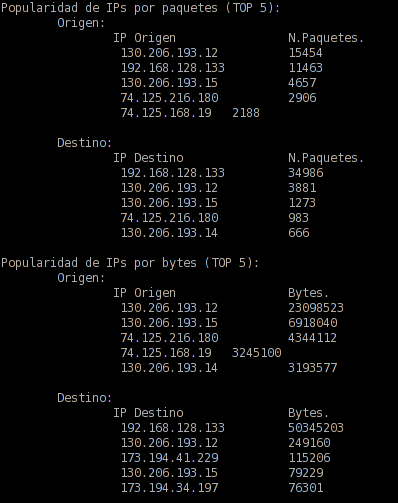
\includegraphics[width=0.8\textwidth]{popularidadIP.png}
\caption{Popularidad de direcciones IP.}
\label{fig:popIP}
\end{figure}

Como se puede observar, la popularidad en paquetes y en bytes no tiene por qué coincidir. Esto es obvio dado que se pueden enviar o recibir paquetes de distintos tamaños, particularmente, de entre 54 y 1514 bytes. Por ejemplo, si una dirección o puerto envía diez asentimientos (ACK) estará enviando diez paquetes de 54 bytes (el tamaño mínimo de la trama ethernet), que será menor en tamaño que un paquete de 1514 bytes.

%Inclusion de imagen.
\begin{figure}[H]
\centering
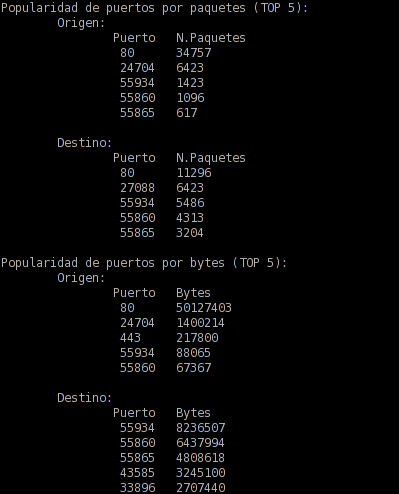
\includegraphics[width=0.8\textwidth]{popularidadPuertos.png}
\caption{Popularidad de puertos.}
\label{fig:popPuertos}
\end{figure}

\subsection{Tamaños de los paquetes}
Para analizar la variable \textit{tamaño del paquete capturado} se han realizado un histograma (\textbf{Figura \ref{fig:tam_hist}}) y un ECDF (\textbf{Figura \ref{fig:tam_ecdf}}) de dicha variable sobre la traza.

%Inclusion de imagen.
\begin{figure}[H]
\centering
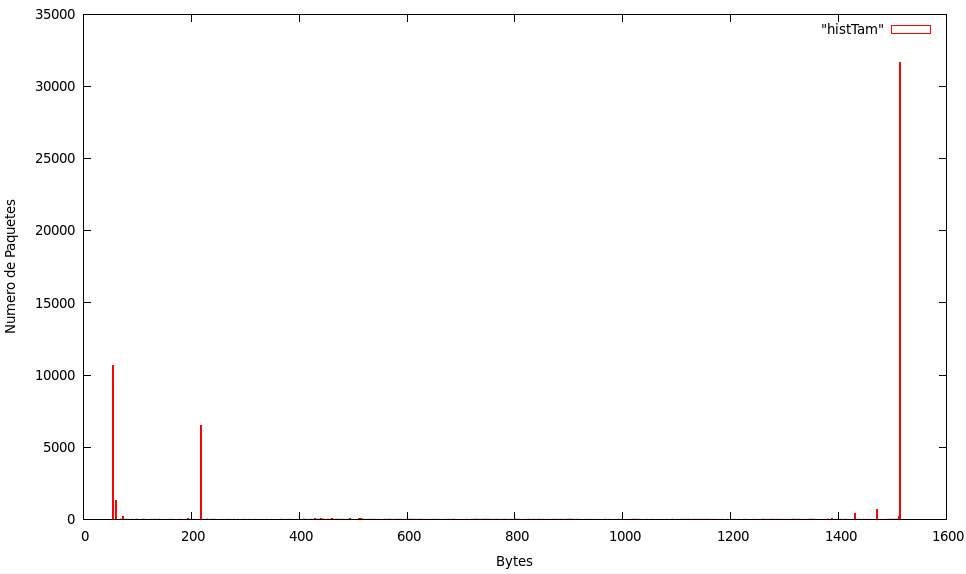
\includegraphics[width=0.8\textwidth]{tam_hist.png}
\caption{Histograma de tamaños de paquetes.}
\label{fig:tam_hist}
\end{figure}

En el histograma puede observarse que la mayoría de paquetes tienen un tamaño de 54, 218 o 1514 bytes.

%Inclusion de imagen.
\begin{figure}[H]
\centering
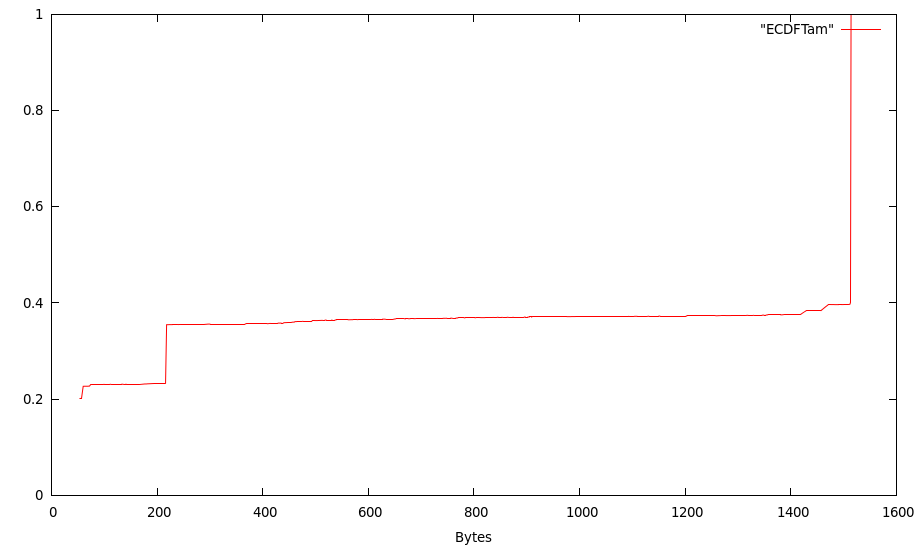
\includegraphics[width=0.8\textwidth]{tam_ecdf.png}
\caption{ECDF de tamaños de paquetes.}
\label{fig:tam_ecdf}
\end{figure}

El ECDF nos muestra una información similar, se puede comprobar que las subidas en el mismo corresponden con los tamaños 54, 218 y 1514 bytes vistos en el histograma.
\\\\
Este resultado se obtiene porque los paquetes de la traza corresponden a asentimientos, tráfico UDP y segmentos de datos.

Los paquetes de 54 bytes se corresponden con asentimientos, que se utilizan para confirmar la recepción de un mensaje (dado que 54 bytes es el tamaño mínimo de una trama ethernet). Por otro lado, los paquetes de 218 bytes corresponden a paquetes de tráfico UDP de esta traza. Y finalmente, los paquetes de 1514 bytes son segmentos de datos, es decir, cuando se quiere enviar una cantidad de datos, se segmentan en varios paquetes ocupando varios de 1514 bytes (el tamaño máximo de una trama ethernet) y el resto de la información se colocará en un paquete del tamaño necesario.

En conclusión, hay una cantidad considerable de paquetes que son asenimientos o tráfico UDP y la gran mayoría del resto de datos que se quieren enviar han sido fragmentados en paquetes de 1514 bytes y en paquetes de tamaño variable que contienen el resto de dicha fragmentación.

\subsection{Ancho de banda a nivel 2 (Throughput)}
Tras analizar el ancho de banda a nivel 2 cada segundo por sentido asumiendo que la dirección Ethernet origen es \textit{00:55:22:af:c6:37} y descartando el tráfico broadcast obtenemos una figura con la representación del throughput (\textbf{Figura \ref{fig:throughput}})

%Inclusion de imagen.
\begin{figure}[H]
\centering
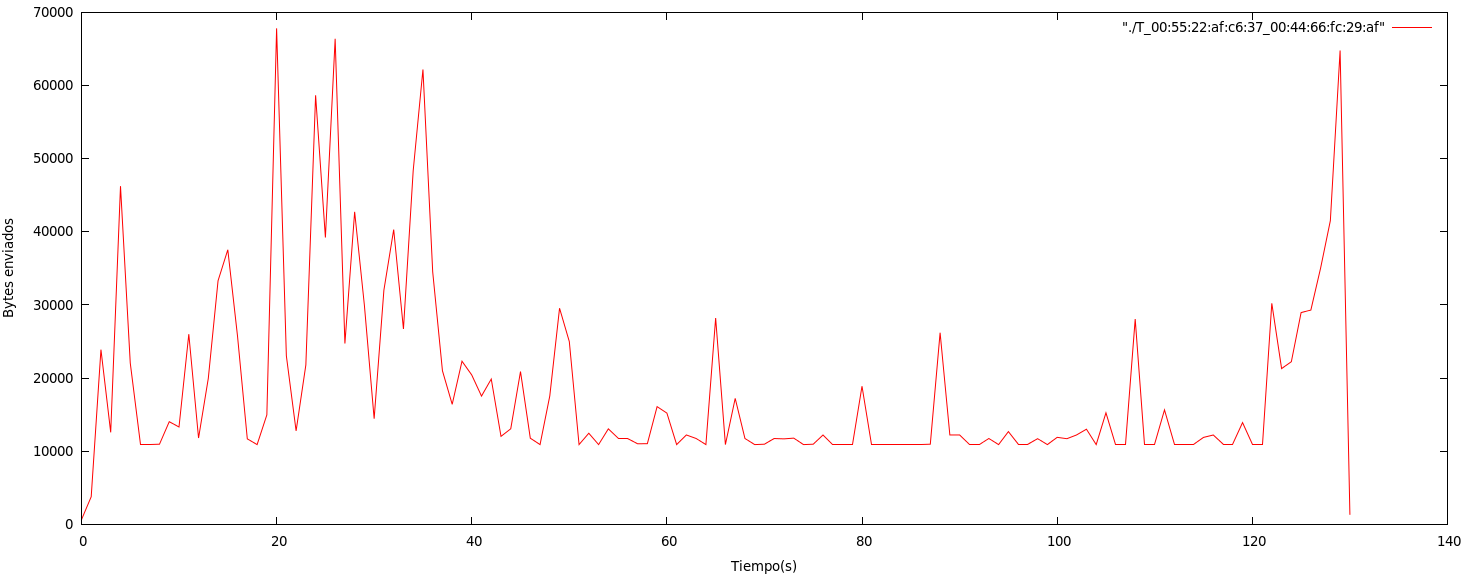
\includegraphics[width=1.0\textwidth]{throughput.png}
\caption{Ancho de banda cada segundo.}
\label{fig:throughput}
\end{figure}

En la gráfica puede observarse que hay una base de tasa de envío de unos 10900 bytes cada segundo, que se corresponden a envíos constantes de paquetes UDP de 218 bytes cada 0,02 segundos aproximadamente ($\frac{218 B}{0,02 s} = 10900\ B/s$).
\\\\
El resto de los saltos de la gráfica pueden deberse a lo que se haya decidido enviar en cada momento, tanto segmentos de datos como asentimientos. El caudal de datos por segundo no sigue una distribución fija pues depende de los paquetes que se envían y del momento en el que se envían, sin embargo, ofrece una visión generalizada de la cantidad de información que se envía en cada momento, así como de las tasas constantes de envío, como en este caso el tráfico UDP.

\subsection{Tiempo entre llegadas de paquetes de un flujo}
Para analizar los tiempos entre llegadas de paquetes de un flujo, se asumirá el flujo UDP con puertos de origen y destino 24704 y 27088 respectivamente. Se obtienen en este caso el histograma (\textbf{Figura \ref{fig:flujo_hist}}) y el ECDF (\textbf{Figura \ref{fig:flujo_ecdf}}) correspondientes.

%Inclusion de imagen.
\begin{figure}[H]
\centering
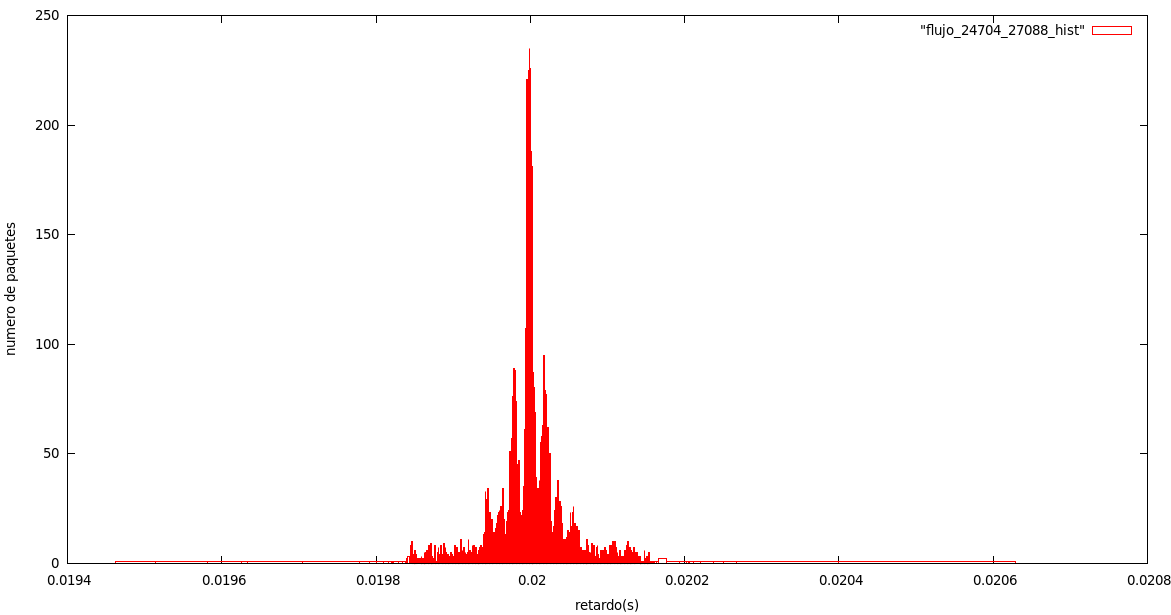
\includegraphics[width=0.8\textwidth]{flujo_hist.png}
\caption{Histograma del tiempo entre llegadas de paquetes del flujo.}
\label{fig:flujo_hist}
\end{figure}

El histograma muestra como el tiempo de llegadas entre paquetes se concentra en 0,02 segundos.

%Inclusion de imagen.
\begin{figure}[H]
\centering
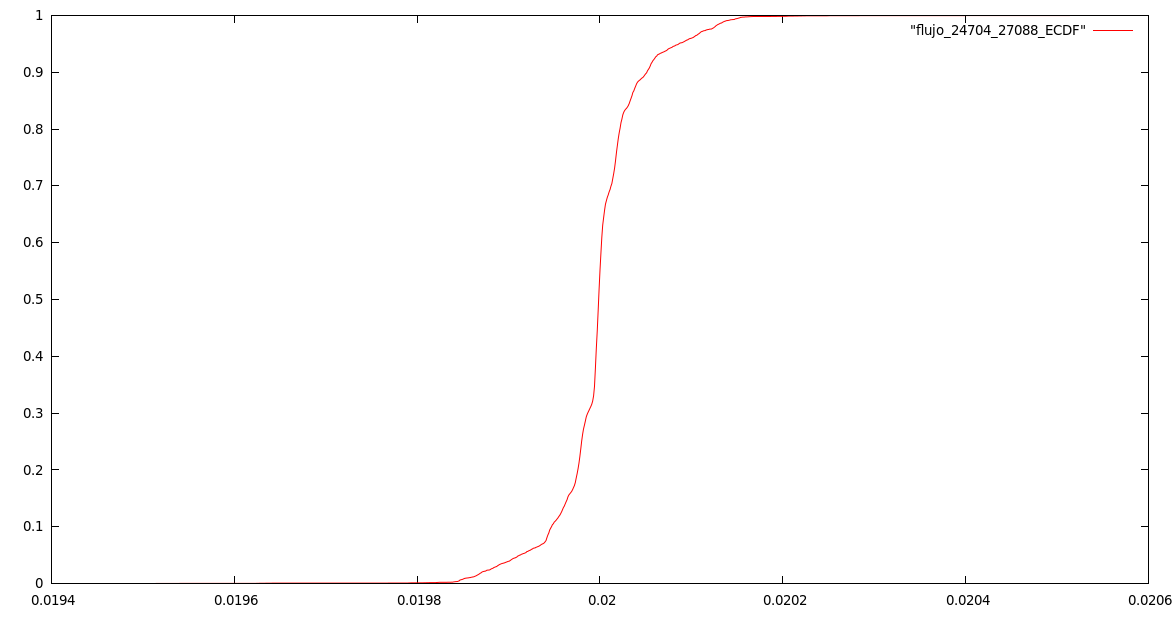
\includegraphics[width=1.0\textwidth]{flujo_ecdf.png}
\caption{ECDF del tiempo entre llegadas de paquetes del flujo.}
\label{fig:flujo_ecdf}
\end{figure}

En el ECDF se observa como el salto en el valor 0,02 de los segundos es muy pronunciado, lo que indica una baja dispersión con respecto a este valor.

En conclusión, en el flujo analizado, se obtiene un tiempo de llegadas entre paquetes centrado y muy próximo a 0,02 segundos en todos los casos, lo que podría atribuirse a una tasa de recibo muy constante y por tanto un Jitter bajo. En los casos en los el Jitter fuera alto, la tasa de recibo no sería constante, sino que sufriría altibajos y el tiempo entre llegadas de paquetes se dispersaría más de su media.

%Apendice
\clearpage
\appendix
\renewcommand\appendixname{Anexo}
\section{Manual de utilización del programa}
\label{sec:manual}
En esta sección se ofrece una breve explicación sobre la utilización del programa implementado.
\subsection{Compilación}
Para compilar el programa se proporciona un fichero Makefile, existen tres opciones equivalentes para la compilación del mismo utilizando el programa make:
\begin{itemize}
\item \textbf{make all} compila el programa y le da el nombre \textit{practica3}
\item \textbf{make practica3} compila el programa y le da el nombre \textit{practica3}
\item \textbf{make main} compila el programa y le da el nombre \textit{main}
\end{itemize}

Para limpiar los archivos generados por la compilación, basta con ejecutar \textbf{make clean}.

\subsection{Ejecución}
Para ejecutar el programa se utiliza la siguiente estructura:

\begin{center}
\textbf{./practica3 INTERF $[<$filtro$>$ $<$dato a filtrar$>]$}
\end{center}

\noindent Donde:\\
\textbf{INTERF} es el fichero pcap o interfaz ethernet (ethX con $X \in [0,9]$).\\
\textbf{$[<$filtro$>$ $<$dato a filtrar$>]:$} puede ser:\\
\indent -ipo x.x.x.x : filtro de IP de origen x.x.x.x ($x \in [0, 255]$)\\
\indent -ipd x.x.x.x : filtro de IP de destino x.x.x.x ($x \in [0, 255]$)\\
\indent -po x : filtro de puerto de origen x ($x \in [0,65536]$)\\
\indent -pd x : filtro de puerto de destino x ($x \in [0,65536]$)\\
\indent -etho xx:xx:xx:xx:xx:xx : filtro de MAC origen ($xx \in [00,FF]$)\\
\indent -ethd xx:xx:xx:xx:xx:xx : filtro de MAX destino ($xx \in [00,FF]$)\\

Se pueden aplicar varios filtros a la vez y el orden de los mismos no se tiene en cuenta.
Si un filtro IP es 0.0.0.0, un filtro de puertos es 0, o un filtro ethernet es 00:00:00:00:00:00 se considerará inexistente, es decir, no se aplicará dicho filtro.

\subsection{Organización de resultados}
Los resultados del programa se oraganizan de la siguiente forma:
\begin{itemize}
\item En la carpeta \textbf{ECDFtamanyos} encontramos tanto el histograma como el ECDF de la variable \textit{tamaño de los paquetes leídos}.
\item En la carpeta \textbf{throughput} encontramos archivos con el formato\\ T$\_$MACorigen$\_$MACdestino que contienen la representación del ancho de banda. En cada fila encontramos dos columnas: segundo y cantidad de bytes enviados durante ese segundo en el sentido MACorigen $\longrightarrow$ MACdestino.
\item En la carpeta \textbf{flujos} tanto un ECDF como un histograma para cada par de puertos en cada sentido que analizan la variable \textit{tiempo de llegada entre paquetes}.
\end{itemize}

El histograma de la variable \textit{tamaño de los paquetes leídos} tiene dos columnas, la primera indica el tamaño de paquete y la segunda el número de paquetes enviados con ese tamaño.

El histograma de la variable \textit{tiempo de llegada entre paquetes} tiene dos columnas, la primera indica el tiempo de llegada entre paquetes y la segunda el número de paquetes que han llegado en ese intervalo (aproximado a la cienmilésima).

\end{document}